\subsection{Subprocesso de Medição e Análise}

Relembrando que o GQM é uma abordagem \textit{top-down} orientado a metas para a mensuração de produtos e processos de software, ou seja, é um processo para definição e interpretação de métricas de software. \cite{junior}

\begin{figure}[H]
	\centering
  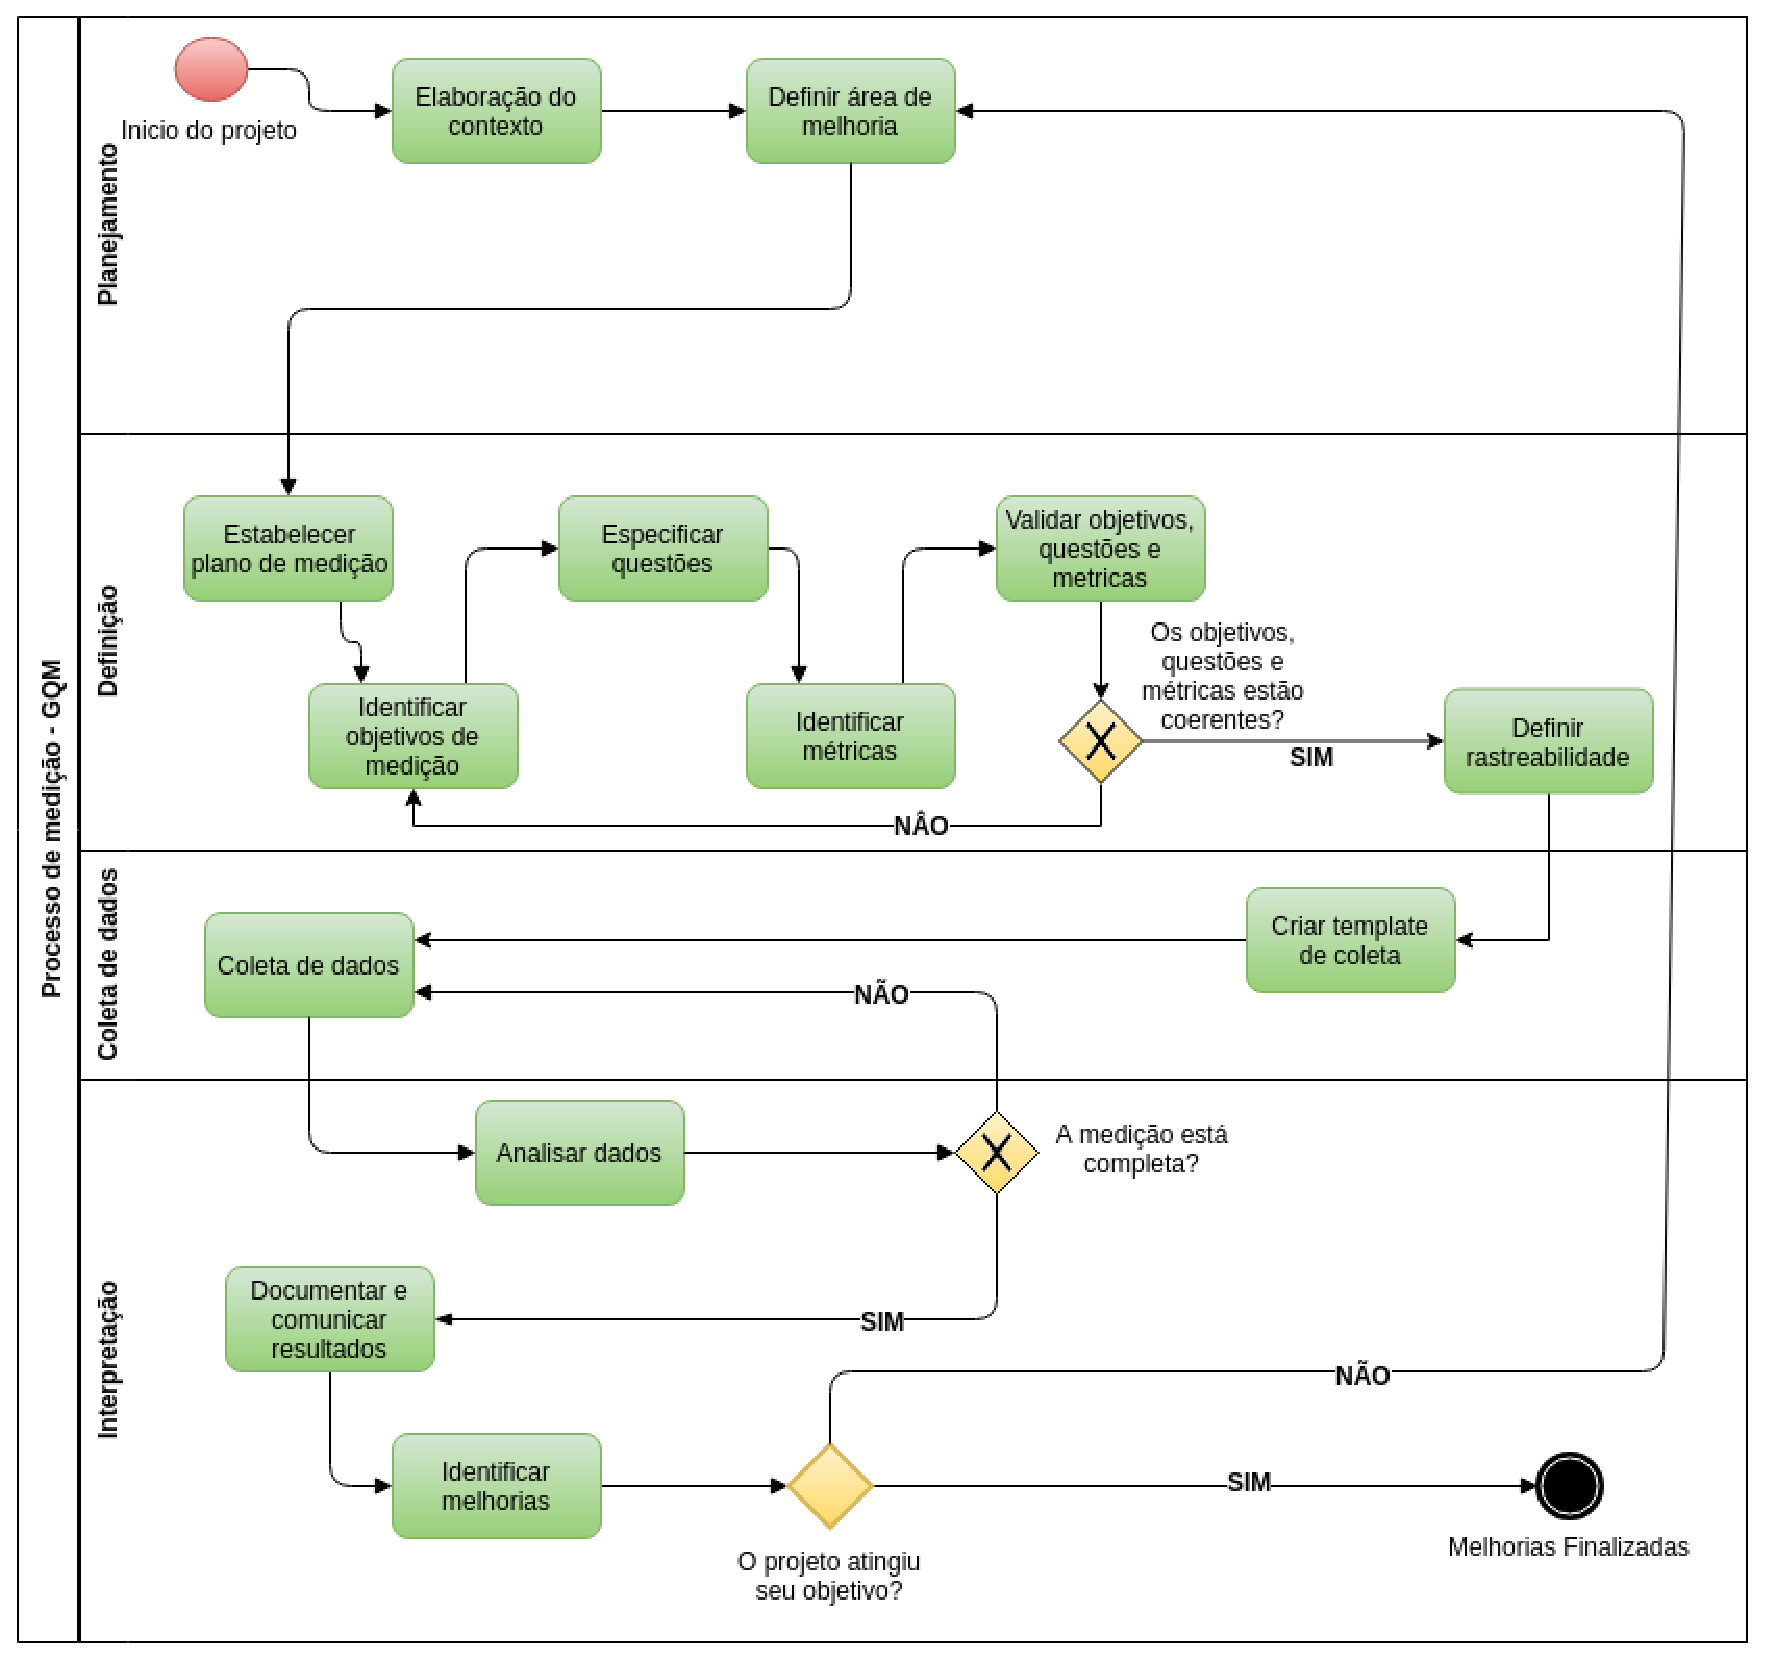
\includegraphics[keepaspectratio=true,scale=0.5]{figuras/processo_gqm.eps}
  \caption[Subprocesso de Medição e Análise (GQM).]{Subprocesso de Medição e Análise (GQM). Fonte: Autor}
	\label{fig:gqm}
\end{figure}

\begin{itemize}
  \item \textbf{Elaboração do contexto}:
  \begin{itemize}
    \item \textbf{Descrição}: Identificar e elaborar o contexto na qual o GQM será aplicado.
    \item \textbf{Entradas}: N/A
    \item \textbf{Saídas}: Inicio do plano de medição
  \end{itemize}
  \item \textbf{Definir área de melhoria}:
  \begin{itemize}
    \item \textbf{Descrição}: Selecionar melhorias a serem implantadas
    \item \textbf{Entradas}: Plano de medição e feedbacks anteriores
    \item \textbf{Saídas}: Plano de medição refinado
  \end{itemize}
  \item \textbf{Estabelecer Plano de Medição}:
  \begin{itemize}
    \item \textbf{Descrição}: Essa etapa é criado ou refinado o plano de medição.
    \item \textbf{Entradas}: Plano de medição se houver
    \item \textbf{Saídas}: Plano de medição refinado
  \end{itemize}
  \item \textbf{Identificar objetivos de medição}:
  \begin{itemize}
    \item \textbf{Descrição}: Essa etapa é identificado os objetivos de medição de forma clara e estruturada.
    \item \textbf{Entradas}: Plano de medição
    \item \textbf{Saídas}: Plano de medição refinado com os objetivos
  \end{itemize}
  \item \textbf{Especificar questões}:
  \begin{itemize}
    \item \textbf{Descrição}: Identificar as questões relacionadas aos objetivos propostos
    \item \textbf{Entradas}: Plano de medição com os objetivos
    \item \textbf{Saídas}: Plano de medição refinado com as questões
  \end{itemize}
  \item \textbf{Identificar Métricas}:
  \begin{itemize}
    \item \textbf{Descrição}: Associar um conjunto de dados a cada questão de forma a respondê-la quantitativamente
    \item \textbf{Entradas}: Plano de medição com os objetivos e questões definidos
    \item \textbf{Saídas}: Plano de medição refinado com as métricas
  \end{itemize}
  \item \textbf{Validar objetivos, questões e métricas}:
  \begin{itemize}
    \item \textbf{Descrição}: Verificar a consistência e completude das métricas em relação ao objeto que desejamos medir
    \item \textbf{Entradas}: Plano de medição com os objetivos, questões e métricas definidas
    \item \textbf{Saídas}: N/A
  \end{itemize}
  \item \textbf{Definir Rastreabilidade}:
  \begin{itemize}
    \item \textbf{Descrição}: Definir a rastreabilidade das métricas com suas respectivas questões e objetivos.
    \item \textbf{Entradas}: Plano de medição com as métricas, questões e objetivos
    \item \textbf{Saídas}: Plano de medição refinado com a rastreabilidade.
  \end{itemize}
  \item \textbf{Criar template de coleta}:
  \begin{itemize}
    \item \textbf{Descrição}: O template de coleta será o mesmo template utilizado para documentar o resultado da sprint,
    já que a coleta será por sprint
    \item \textbf{Entradas}: N/A
    \item \textbf{Saídas}: N/A
  \end{itemize}
  \item \textbf{Coleta de dados}:
  \begin{itemize}
    \item \textbf{Descrição}: A cada sprint será coletado em paralelo com o desenvolvimento as métricas definidas no plano
    de medição.
    \item \textbf{Entradas}: N/A
    \item \textbf{Saídas}: Dados coletados nas suas respectivas ferramentas
  \end{itemize}
  \item \textbf{Análise de dados}:
  \begin{itemize}
    \item \textbf{Descrição}: Com os dados coletados pelas ferramentas de análise estática de código e testes, será
    analisado o resultado com o resultado esperado no plano de medição.
    \item \textbf{Entradas}: N/A
    \item \textbf{Saídas}: N/A
  \end{itemize}
  \item \textbf{Documentar e comunicar resultados}:
  \begin{itemize}
    \item \textbf{Descrição}: Ao final da sprint na revisão e retrospectiva será documentado o resultado da sprint com as
    métricas coletadas.
    \item \textbf{Entradas}: Métricas coletadas e analisadas
    \item \textbf{Saídas}: Resultado da sprint.
  \end{itemize}
  \item \textbf{Identificar melhorias}:
  \begin{itemize}
    \item \textbf{Descrição}: Com os resultados coletados, analisados e documentados será identificado o que pode melhorar
    para a próxima iteração.
    \item \textbf{Entradas}: Resultado da Sprint
    \item \textbf{Saídas}: Melhorias.
  \end{itemize}
\end{itemize}
